\chapter{Hardware}%
    \label{chp:Hardware}
	
	A planta possui uma eletrônica embarcada responsável por fazer a alimentação dos componentes, sensoriamento dos graus de liberdade, e atuação dos motores. Dua baterias são utilizadas para fornecer energia ao dispositivo. A integração do microprocessador com os componentes da planta, bem como dos componentes entre sí, pode ser vista no diagrama elétrico na Figura \ref{img:diagrama}.
	
	\begin{figure}[h]
        \centering
        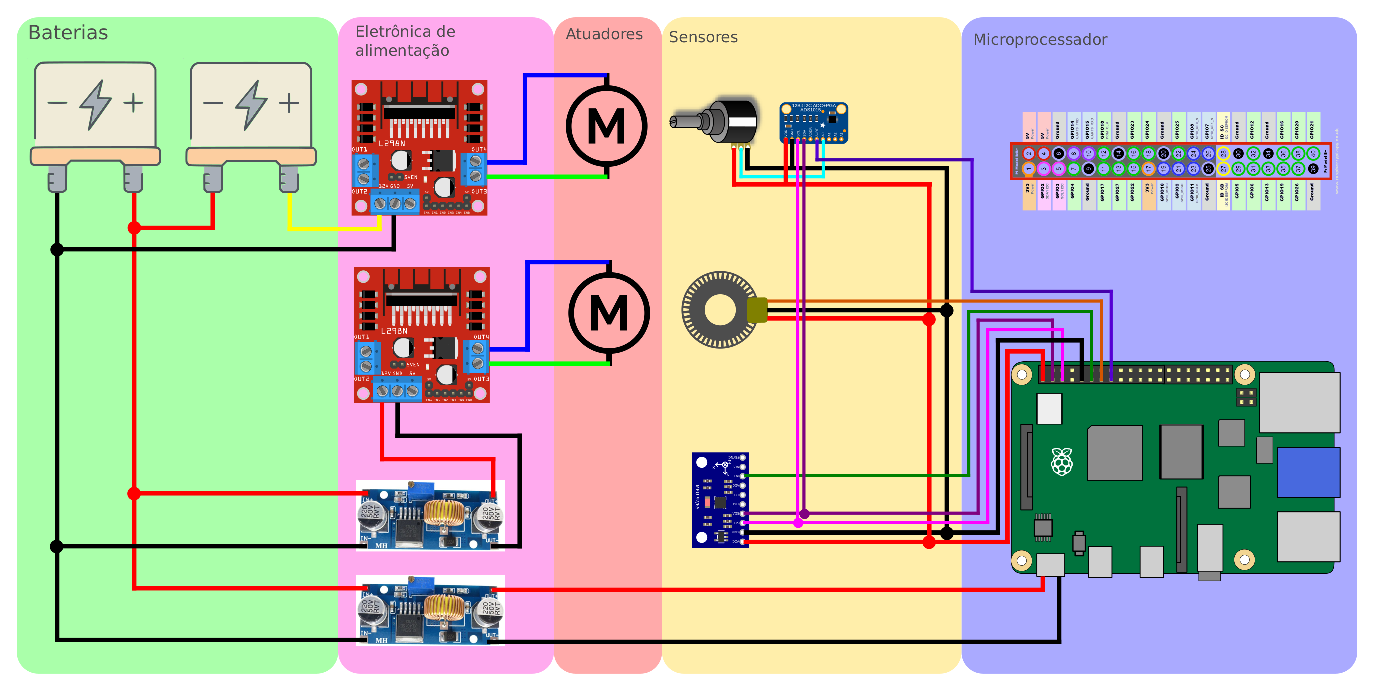
\includegraphics[width=\columnwidth]{Imagens/cap2/montagem3.eps}
        \caption{Diagrama elétrico da planta.}
        \label{img:diagrama}
    \end{figure}
    
    \section{Microprocessador}
	    
	    O microcontrolador proposto para a realização deste trabalho foi o Raspberry Pi 4 Model B. Ele possuí um processador \textit{Broadcom BCM2711} que possuí quatro núcleos \textit{Cortex-A72} rodando a uma frequência de $1.5 GHz$ cada, e possuem arquitetura \textit{ARM64}. Ele possuí um barramento de pinos que permite a conexão com sensores e outros dispositivos eletrônicos através de diversos protocolos, como \textit{PWM}, \textit{I2C}, \textit{SPI}, etc. A tensão de alimentação da placa é de $5V$.
	
    	\begin{figure}[h]
            \centering
            \includegraphics[width=7cm]{Imagens/cap2/rasp2.jpg}
            %\caption{Raspberry Pi 4 com \textit{case} de proteção e resfriamento.}
            \caption{Raspberry Pi 4 model B.}
            \label{img:theta}
        \end{figure}
	
	    A \textit{GPIO} do \textit{Raspberry} trabalha com tensão $3.3V$, por isso os sensores serão alimentados com a mesma tensão. O \textit{Raspberry} fornece um pino de saída com essa tensão, que é usado para alimentar os sensores.
    
    \section{Sensores}
    
    	Para realizar o sensoriamento da inclinação da planta em relação a gravidade é usado o sensor inteligente \textit{MPU-9250}, que contém vários sensores embutidos: 3 Acelerômetros, 3 Giroscópios e 3 Magnetômetros, totalizando 9 graus de liberdade. Sendo que cada trio de sensores são perpendiculares entre si. Além disso ele possui um \textit{DMP (Digital Motion Processor)}, que é um microprocessador que realiza a fusão de sensores a fim de obter a orientação espacial do conjunto. Como o sensor é fixo em relação ao corpo da planta, é possível obter a inclinação em relação a gravidade através da orientação espacial que o sensor fornece. Uma foto do sensor pode ser vista na Figura \ref{img:mpu}.
    	
    	\begin{figure}[h]
            \centering
            \includegraphics[width=4cm]{Imagens/cap2/mpu.png}
            \caption{Foto do sensor \textit{MPU-9250}}
            \label{img:mpu}
        \end{figure}
        
    	O eixo de direção da roda dianteira possui um servo motor \textit{TowerPro MG995} acoplado, composto por um motor, uma redução de engrenagens, e um potenciômetro integrado. O potenciômetro tem 3 vias e uma resistência interna de $10k$. Originalmente este servo vem com um uma placa de circuito integrado que realiza a comunicação com um micro-controlador e o controle do eixo de saída, mas tal placa foi retirada para o controle ser feito diretamente pelo microcontrolador. O potenciômetro, por sua vez, é conectado a um conversor analógico digital \textit{Ads1115} que converte a tensão de saída em uma faixa de 16 bits, e envia a leitura para o microcontrolador.
	
    	\begin{figure}[h]
            \centering
            \includegraphics[width=4cm]{Imagens/cap2/995.png}
            \caption{Foto do servomotor \textit{TowerPro MG995}.}
            \label{img:theta}
        \end{figure}
        
        \begin{figure}[h]
            \centering
            \includegraphics[width=4cm]{Imagens/cap2/ads.png}
            \caption{Foto do conversor analógico digital \textit{Ads1115}.}
            \label{img:theta}
        \end{figure}
        
    	O sensoriamento da velocidade tangencial é realizado por um encoder óptico \textit{OPB-991T51}. Ele é composto por um LED infravermelho, um foto-transistor, e um disco com orifícios. O LED fica alinhado com o foto-transistor, que dependendo da posição angular do disco, impede ou não a passagem do infravermelho. Quando há a passagem de luz o foto-transistor fecha circuito elétrico, e vice-versa. Como o disco do encoder está acoplado a roda traseira, partindo do pressuposto que a roda gira apenas em um sentido, é possível saber aproximadamente quantos graus a roda girou através do sinal elétrico. Logo, é possível um microcontrolador calcular a velocidade tangencial dividindo a variação angular pela variação de tempo. Uma foto do conjunto do encoder pode ser vista na Figura \ref{img:encoder},
    	
    	\begin{figure}[h]
            \centering
            \includegraphics[width=8cm]{Imagens/cap2/foto-encoder.jpg}
            \caption{Foto da vista lateral esquerda da planta - Encoder Óptico \textit{OPB-991T51}.}
            \label{img:encoder}
        \end{figure}
    
    \section{Atuadores}
    
	    A roda traseira tem também um atuador acoplado a ela por intermédio de uma polia-correia. O motor é de corrente continua de ímã permanente, como explicado na sessão \ref{sec:motorcc} e este pode receber uma tensão máxima de $24V$. Os outros parâmetros referentes ao motor, bem como da polia-correia, serão fornecidos na sessão \ref{sec:modelagemvelocidade}. Uma foto do motor acoplado a polia pode ser visto na Figura \ref{img:motor-polia}.
	
    	\begin{figure}[h]
            \centering
            \includegraphics[width=8cm]{Imagens/cap2/foto-motor-polia.jpg}
            \caption{Foto da vista lateral direita da planta - Motor e Polia.}
            \label{img:motor-polia}
        \end{figure}
	    
	    O motor do servo motor acoplado ao eixo de direção, de acordo com a fabricante, suporta uma tensão máxima de $7,2V$. Novamente, os outros parâmetros referentes ao motor, bem como da redução, serão fornecidos na sessão \ref{sec:modelagemvangulo}.
	
	\section{Eletrônica de alimentação e Baterias}
	    
	    Ambos motores são alimentados por intermédio de uma ponte H \textit{LN298} para cada. Elas são responsável por receber um sinal \textit{PWM} cada do microcontrolador, e aplicar esse sinal em seu respectivo motor.
	
    	\begin{figure}[h]
            \centering
            \includegraphics[width=5cm]{Imagens/cap2/ln298.png}
            \caption{Foto da ponte H \textit{LN298}}
            \label{img:theta}
        \end{figure}
    
	    As baterias que alimentam a planta são de polímero de lítio, com tensão nominal de $12,6V$. Cada célula de carga trabalha com uma tensão que varia de $3.5V$ quando descarregadas a $4,2V$ quando em carga máxima. Como cada bateria possuí 3 células, a tensão de trabalho de cada bateria varia de $12,6V$ a $10,5V$. As duas estão associadas em série, totalizando um tensão aproximada de $24V$, tendo disponível o terminal intermediário entre elas com tensão de $12V$.
	
    	\begin{figure}[h]
            \centering
            \includegraphics[width=5cm]{Imagens/cap2/bateria.jpg}
            \caption{Foto do tipo de bateria de polímero de lítio utilizado.}
            \label{img:theta}
        \end{figure}
	    
	   Como alguns dispositivos tem tensão diferente da bateria, faz-se necessário abaixar essa tesão para determinados dispositivos. Para isso vem acoplados na planta dois conversores de tensão \textit{Step-down} \textit{Xl4015} que convertem a tensão da bateria para o valor necessário. O primeiro é ajustado em $7V$ para alimentar a ponte-H que alimenta o servomotor, enquanto a ponte h que alimenta o motor traseiro recebe tensão direta vinda da bateria. E o outro conversor é ajustado para uma saída de $5V$ para alimentar o microprocessador.
	
    	\begin{figure}[h]
            \centering
            \includegraphics[width=4cm]{Imagens/cap2/xl.jpg}
            \caption{Foto do conversor de tensão \textit{Xl4015}.}
            \label{img:theta}
        \end{figure}
